\chapter{Preliminary}


\section{Reinforcement Learning \& PPO}

According to \cite{Fran_ois_Lavet_2018_rlintro}, Reinforcement Learning can be defined as \enquote{the area of machine learning that deals with sequential decision-making}; it is a method of training an agent to learn a specific behaviour by interacting and observing the environment that it exists inside of. With each action performed by the agent which affects the environment, it can be rewarded or punished so that with each iteration it can adapt its behaviour to be slightly more similar to the desired behaviour. 

\cite{Fran_ois_Lavet_2018_rlintro} defines the general Reinforcement Learning problem as a \enquote{discrete time stochastic control process where an agent interacts with its environment in the following way: the agent starts, in a given state within its environment $s_0 \in \gS$, by gathering an initial observation $\omega_0 \in \Omega$. At each time step $t$, the agent has to take an action $a_t \in \gA$. [\dots]. it follows three consequences: (i) the agent obtains a reward $r_t \in \gR$, (ii) the state transitions to $s_{t+1} \in \gS$, and (iii) the agent obtains an observation $\omega_{t+1} \in \Omega$}. Because of this, Reinforcement Learning can be modeled as a Markov Decision Process (MDP). According to \cite{Bellman_MDP}, a MDP is a 4-tuple $(\gS, \gA, T, R)$ where:
\begin{itemize}
    \item [$\gS$]: is the state space
    \item [$\gA$]: is the action space
    \item [$T$]: is the transition function; it is defined as $T: \gS \times \gA \times \gS \rightarrow [0, 1]$, and represents the probability that an action $a \in \gA$ will lead from state $s \in \gS$ to state $s' \in gS$
    \item [$R$]: is the reward function; it is defined as $R: \gS \times \gA \times \gS \rightarrow \gR$, and represents the reward obtained when moving from state state $s \in \gS$ to state $s' \in gS$ because of action $a \in \gA$
\end{itemize}

Another notion of Reinforcement Learning is the policy, which shows how an agent selects the action that it will take. It can be defined as $\pi: \gA \times \gS \rightarrow [0, 1]$, where $\pi(a, s)$ is the probability of action $a$ being chosen while in state $s$.

To solve a Reinforcement Learning problem there are multiple ways, such as model-based methods, value-based methods, policy gradient methods, etc. The ones that are important for this paper are the methods with policy gradients, since those are the ones that will be used. Policy gradient methods learn a parameterized policy and optimize it directly. The policy can be defined as 
\begin{equation} \label{policy_eq:1}
    \pi_{\theta} (a | s) = Pr\{a_t = a | s_t = s, \theta_{t} = \theta\}
\end{equation}
where $\theta \in \sR^{d'}$ is the policy's parameter vector.




According to \cite{schulman2017ppo} \enquote{Policy gradient methods work by computing an estimator of the policy gradient and plugging it into a stochastic gradient ascent algorithm. The most commonly used gradient estimator has the form 

\begin{equation}
    \hat{g} = \hat{\mathbb{E}}_{t} [\nabla_{\theta} log \pi_{\theta}(a_t | s_t) \hat{A}_{t}]    
\end{equation}
where $\pi_{\theta}$ is a stochastic policy and $\hat{A}_{t}$ is an estimator of the advantage function at timestep $t$.}

$\hat{\mathbb{E}}_{t}$ is the expectation which is used in an algorithm that alternates between optimization and sampling, and which indicates the empirical average over a finite batch of samples. Implementations utilizing automatic differentiation software operate by creating an objective function, the gradient of which serves as the policy gradient estimator. The estimator $\hat{g}$ is derived through the differentiation of the objective

\begin{equation}
    L^{PG} (\theta) = \hat{\mathbb{E}}_{t} [log \pi_{\theta}(a_t | s_t) \hat{A}_{t}]
\end{equation}

\paragraph{}
Proximal policy optimization (PPO) works by sampling the data obtained from interacting with the environment and then optimizes the objective function with stochastic gradient ascent

\begin{equation}
    r_t(\theta) = \frac{\pi_{\theta} (a_t | s_t)}{\pi_{\theta_{\text{old}}} (a_t | s_t)}
\end{equation}

\begin{equation}
    L(\theta) = \hat{\mathbb{E}}_{t} [min(r_t(\theta) \hat{A}_{t}, clip(r_t(\theta), 1-\epsilon, 1+\epsilon) \hat{A}_{t})]
\end{equation}
where $r_t(\theta)$ is the probability ratio. It can be seen that the probability function is clipped in order for the surrogate objective to be modified.

The PPO algorithm that uses fixed-length trajectory segments as defined in \cite{schulman2017ppo} can be seen in Alogrithm \ref{alg:ppo}

\begin{algorithm}
    \caption{PPO, Actor-Critic Style}\label{alg:ppo}
    \begin{algorithmic}
    \For{iteration $ = 1, 2, \dots $}
        \For{actor $ = 1, 2, \dots, N$}
            \State Run policy $\pi_{\theta_{\text{old}}}$ in environment for $T$ timesteps
            \State Compute advantage estimates $\hat{A}_{1}, \dots, \hat{A}_{T}$
        \EndFor
        \State Optimize surrogate $L$ wrt $\theta$, with $K$ epochs and minibatch size $M \leq NT$
        \State $\theta_{\text{old}} \gets \theta$
    \EndFor
    \end{algorithmic}
\end{algorithm}

At each iteration, each of the $N$ actors collect $T$ timesteps of data, then the surrogate loss is constructed on the $NT$ timesteps of data and optimized witha  minibatch SGD for $K$ epochs.

% sa mai copiez niste cacat pe aici

\section{Unity \& ML-Agents Toolkit}

The environment where the solution will be implemented will be a Unity project consisting of a small level that has different structures an objects, and which contains tanks that can move, shoot, and fight eachother. The project also contains an AI implementation that is based on behaviour trees and genetic algorithms and is described in more detail in \cite{paduraru2019automatic}. The project can be found at \url{https://github.com/AGAPIA/BTreeGeneticFramework}. The level that is contained in the mentioned project, and that will be used for training, can be seen in Figure \ref{photo:tank_training_env}.

\begin{figure}
    \begin{center}
        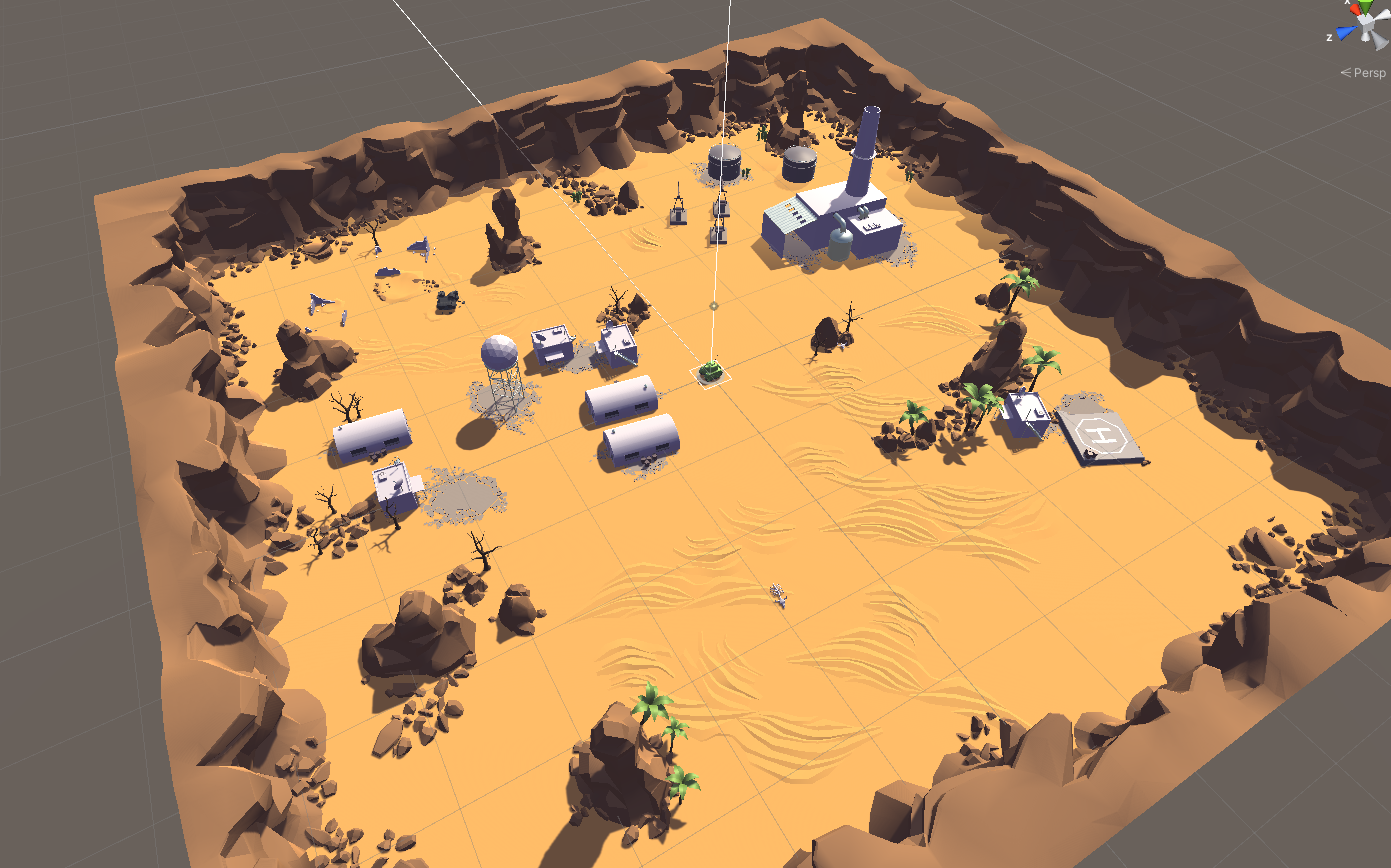
\includegraphics[width=0.9\linewidth]{tanks_4.png}
        \caption{The training environment}
        \label{photo:tank_training_env}
    \end{center}
\end{figure}

The ML-Agents Toolkit is defined as \enquote{an open source project which enables researchers and developers to create simulated environments using the Unity Editor and interact with them via a Python API. The toolkit provides the ML-Agents SDK which contains all functionality necessary to define environments within the Unity Editor along with the core C\# scripts to build a learning pipeline} \cite{juliani2020unityai}. The toolkit also provides implementation in PyTorch for most state-of-the-art reinforcement learning algorithms, including PPO, and several example environments to quickly test the toolkit.

The training hyperparameters for PPO can be configured via a \emph{.yaml} file, and the configurable parameters, according to \cite{mlagents_api_docs}, are:
\begin{itemize}
    \item Gamma ($\gamma$): the discount factor for future rewards
    \item Lambda ($\lambda$): the lambda parameter used when calculating the Generalized Advantage Estimate
    \item Beta ($\beta$): the strength of the entropy regularization
    \item Epsilon ($\epsilon$): the acceptable threshold of divergence between the old and new policies during gradient descent updating
    \item Buffer Size: how many experiences should be collected before we do any learning or updating of the model
    \item Batch Size: the number of experiences used for one iteration of a gradient descent update
    \item Number of Epochs: the number of passes through the experience buffer during gradient descent
    \item Learning Rate: the strength of each gradient descent update step
\end{itemize}

In addition, ML-Agents also provides support for using Recurrent Neural Networks (RNN), in the form of LSTMs (Long short-term memory). This option can be used by setting a flag in the trainer's configuration. It provides two configuration parameters:
\begin{itemize}
    \item Sequence Length: how long the sequences of experiences must be while training
    \item Memory Size: the size of the memory the agent must keep
\end{itemize}

There are 3 entities provided by the ML-Agents SDK:
\begin{itemize}
    \item Sensors, which are used to collect the observations from the environment
    \item Agents, which are components to add the Agent functionality to a Unity GameObject, which enables them to collect observations, decide which action to take by using the observations and execute them, and receive rewards
    \item Academy, which can be defined as a singleton instance that manages agent training and decision making \cite{mlagents_api_docs}
\end{itemize}

The observations that are collected, the actions that should be taken by the agent, and the rewards received by the agent can be implemented manually using the provided \emph{Agent} class.

The ML-Agents Toolkit also has a Python package, \emph{mlagents}, which according to \cite{mlagents_pypi}, provides a set of reinforcement and imitation learning algorithms designed to be used with Unity environments. This package will be used to effectively run the training process, by communicating with the Unity application via a gRPC communication protocol.

% sa bag poze, sa zic ca mlagents imi ofera moduri de a scripta ce obs fac ce pedepse si recompense dau pt agent, modalitate de a antrena si a face inferenta cu ce am antrenat probabil sa iau ceva si de la \cite{juliani2020unityai}